\documentclass{article}
\usepackage{graphicx} % Required for inserting images
\usepackage[a4paper, left=3cm, right=2cm, top=2cm, bottom=2cm]{geometry}
\usepackage{float}
\usepackage{subcaption}  % For subfigure support
\usepackage{subfigure}


\title{Lab3 Report}
\author{Nguyen Thanh Tung - 2440047}
\begin{document}
\maketitle


\begin{figure}[h!]
    \centering
    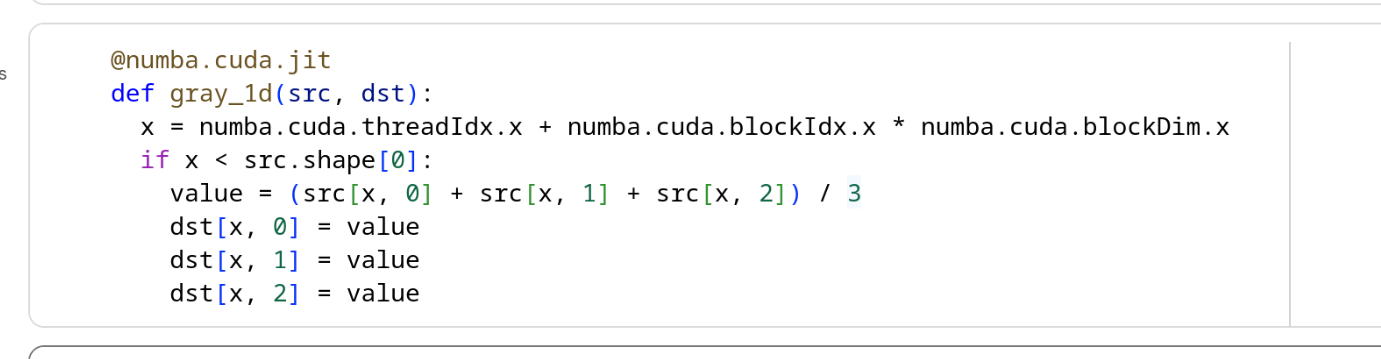
\includegraphics[width=1\linewidth]{impl.png}
    \caption{Kernel implementation}
    \label{fig:kernel}
\end{figure}

\begin{figure}[h!]
    \centering
    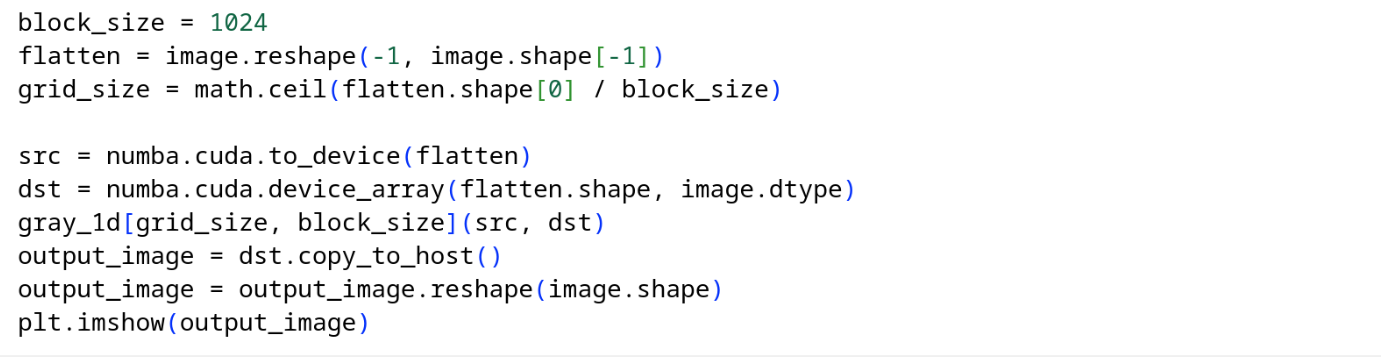
\includegraphics[width=1\linewidth]{run.png}
    \caption{Executing the kernel}
    \label{fig:exec}
\end{figure}


We implemented the kernel as shown in Figure \ref{fig:kernel}. Then we can execute the kernel as in Figure \ref{fig:exec}. In the implementation of the kernel, first we get the "x" position of the current thread in the grid, then we compare it to the image size to make sure it is within the bounds. Then we just simply set the output image channel to the average of the source input channel. We use 1024 (the maximum) block size for the best performance. The grid size is calculated by dividing the total number of pixels by the number of threads per block. We need to flatten the input image and copy it to the device. In addition, we have to allocate the output array. We execute the kernel with the grid size and block size. In the end we copy the output array back to the host and reshape it.


\begin{figure}[h!]
    \centering
    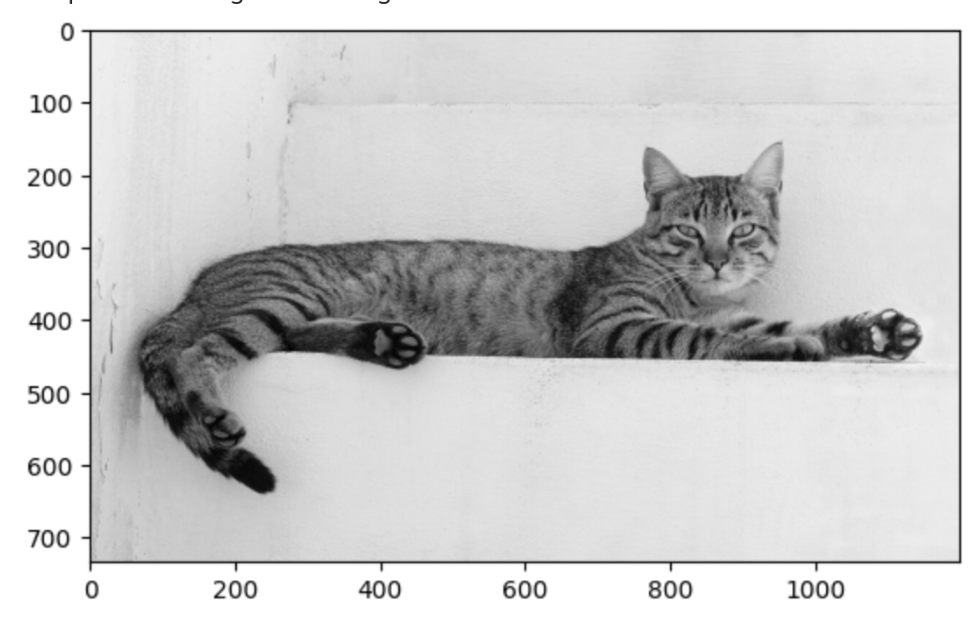
\includegraphics[width=0.5\linewidth]{output.png}
    \caption{Output image}
    \label{fig:placeholder}
\end{figure}


\begin{figure}[h!]
    \centering
    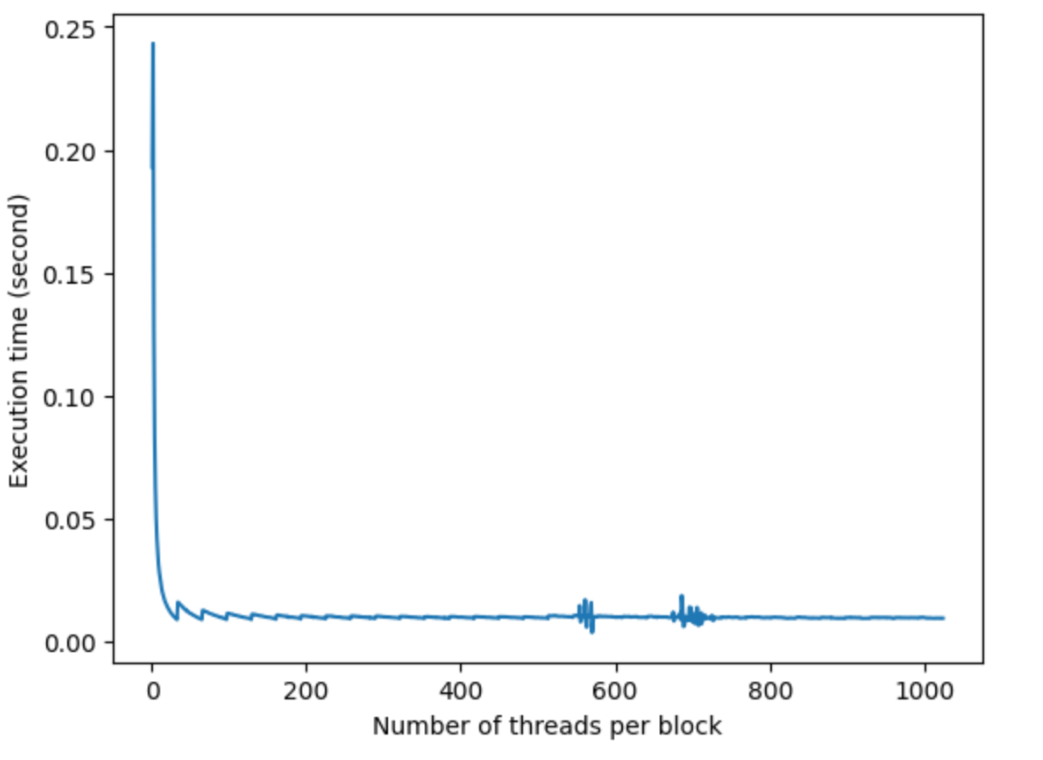
\includegraphics[width=0.5\linewidth]{block_size_plot.png}
    \caption{Effect of block size on execution time}
    \label{fig:placeholder}
\end{figure}

When we increase the block size, the execution time dramatically decreases because we can run more threads concurrently.


\begin{figure}[h!]
    \centering
    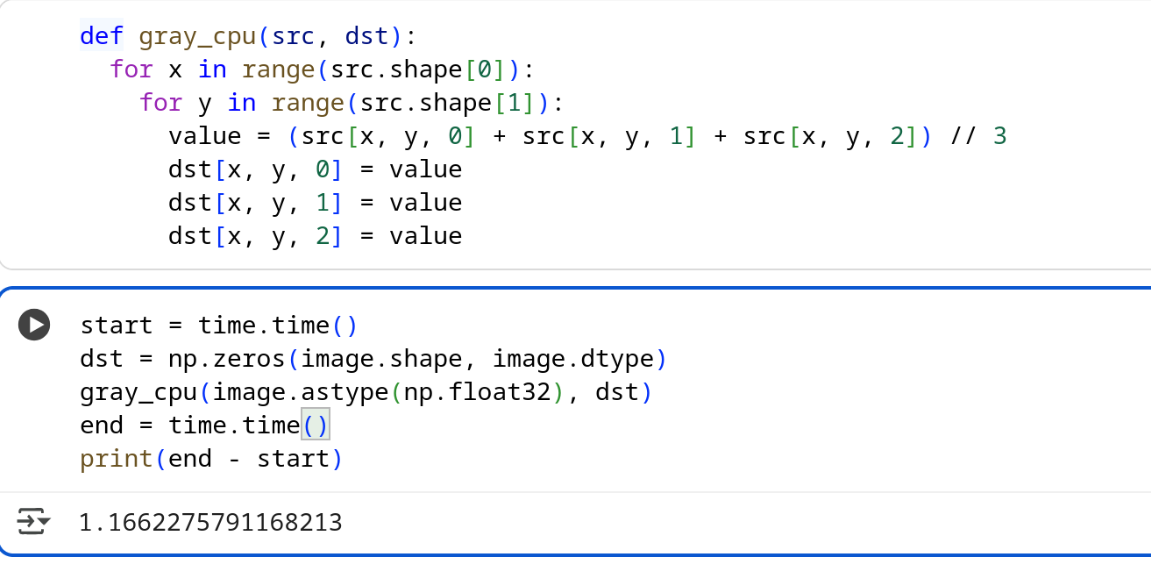
\includegraphics[width=0.5\linewidth]{cpu.png}
    \caption{CPU implementation}
    \label{fig:placeholder}
\end{figure}

The CPU implementation is significantly slower compared to using the GPU.




\end{document}
